\subsection{Visualización efectiva}
\label{visualizacion_efectiva}
La visualización de datos es el conjunto de técnicas usadas para comunicar
datos o información a través de su codificación como objetos visuales
contenidos en gráficos. La meta es comunicar información de forma clara y
eficiente a los usuarios. La visualización efectiva ayuda a los usuarios a
analizar y razonar sobre datos y evidencia, y transforma datos complejos en
datos accesibles, entendibles y utilizables.

El uso de técnicas efectivas de visualización permite entender mejor los datos
y ayuda a descubrir tendencias, revelar ideas, explorar fuentes y contar
historias. En los últimos años la visualización de datos se ha vuelto un área
activa de investigación, enseñanza y desarrollo.

Para este desarrollo nos interesa usar técnicas de visualización de datos para
elaborar cuadros de mando útiles y poder comunicar información de la manera más
adecuada para cada usuario.

La visualización de datos es una herramienta para ayudar al análisis y no un
sustituto de la habilidad analítica. Para lograr una visualización de datos
efectiva es útil contar con conocimiento de negocio, estadística, teoría del
color, psicología, composición gráfica e inteligencia emocional.

Existen muchas formas de presentación de datos, y cada una tiene su propósito
específico. A continuación se explican algunas de ellas:

\subsubsection*{Tabla}
Es un modo de organizar información en filas y columnas que es útil para
comparar valores. A través del uso de colores y explicaciones, se puede hacer
que la información contenida en las mismas sea más fácil de decodificar
(\autoref{fig:representacion_tabla}).

\begin{figure}
  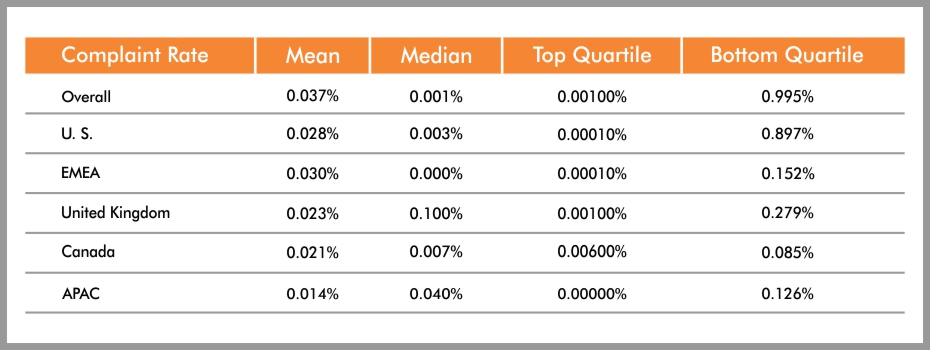
\includegraphics[width=\linewidth]{src/images/01-capitulo-1/representacion_tabla.jpg}
  \caption{Diagrama de representación en forma de tabla}
  \label{fig:representacion_tabla}
\end{figure}

\subsubsection*{Gráfico de barra}
Es una forma de representar gráficamente conjuntos de datos o valores, a través
del uso de barras rectangulares de longitudes proporcionales a los valores
representados. Son útiles para comparar elementos
(\autoref{fig:representacion_barras}).

\begin{figure}
  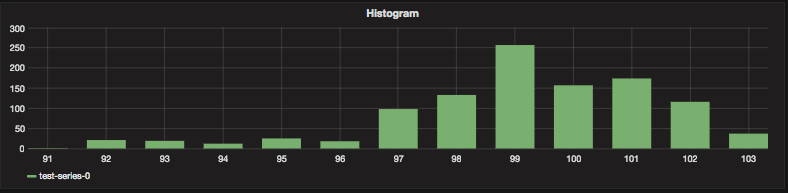
\includegraphics[width=\linewidth]{src/images/01-capitulo-1/representacion_barras.png}
  \caption{Diagrama de representación con barras}
  \label{fig:representacion_barras}
\end{figure}

\subsubsection*{Gráfico de línea}
Es una manera de visualizar información compuesta de una serie de datos
representados por puntos y unidos por segmentos lineales. Este tipo de gráficos
sirve para comprobar de forma sencilla la tendencia de los
datos.(\autoref{fig:representacion_lineas})

\begin{figure}
  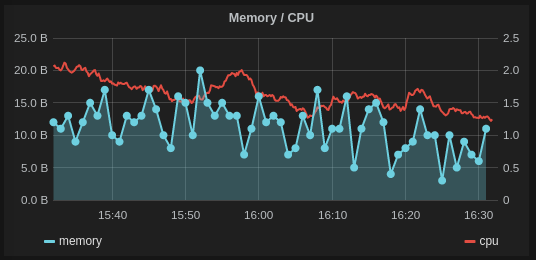
\includegraphics[width=\linewidth]{src/images/01-capitulo-1/representacion_lineas.png}
  \caption{Diagrama de representación con líneas}
  \label{fig:representacion_lineas}
\end{figure}

\subsubsection*{Gráfico circular}
También llamado gráfico de torta o \eng{pie chart}. Es un recurso estadístico
que se utiliza para representar porcentajes o proporciones. Consiste en dividir
a un círculo en secciones coloreadas, donde el tamaño de cada sección es
proporcional al valor que se intenta representar
(\autoref{fig:representacion_circular}).

\begin{figure}
  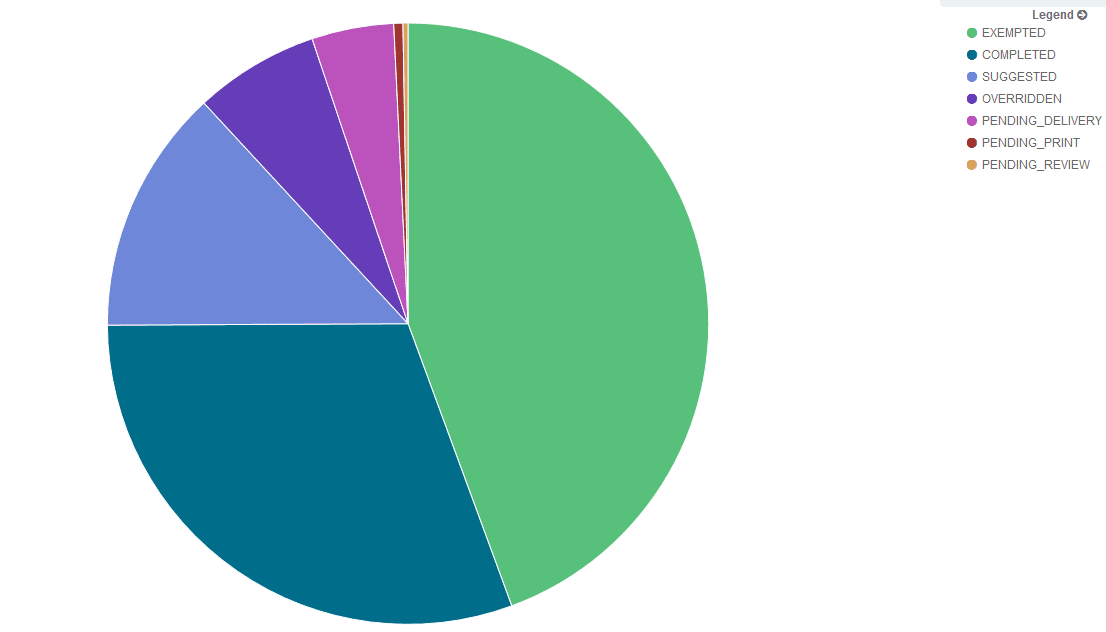
\includegraphics[width=\linewidth]{src/images/01-capitulo-1/representacion_circular.png}
  \caption{Diagrama de representación en forma circular}
  \label{fig:representacion_circular}
\end{figure}

\subsubsection*{Gráfico de dispersión}
También conocidos como \eng{Scatter Plot}, estos gráficos usan valores
numéricos para ambos ejes. Son útiles para mostrar la relación entre distintos
tipos de datos. Los gráficos de burbujas son una variación de este tipo de
gráficos, los puntos pueden ser de distintos tamaños, representando una
dimensión adicional a los datos (\autoref{fig:representacion_dispersion}).

\begin{figure}
  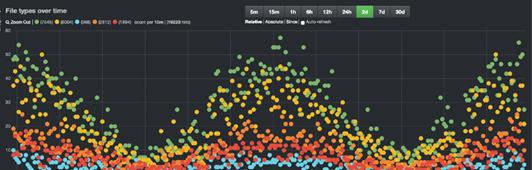
\includegraphics[width=\linewidth]{src/images/01-capitulo-1/representacion_dispersion.jpg}
  \caption{Diagrama de representación de dispersión}
  \label{fig:representacion_dispersion}
\end{figure}

A la hora de mostrar información es importante conocer las distintas maneras de
visualizar información, analizar qué es lo que se quiere transmitir y tener
criterio para decidir la forma en la que se mostrarán los datos.

